\documentclass[11pt]{article}
\usepackage{myz310e-notes}
\usepackage{needspace}
\hypersetup{pdftitle={Training neural networks: backpropagation, regularisation and initialisation},pdfauthor={Emre Onur Kahya},pdfsubject={MYZ 310E Machine Learning in Physics, Fall 2026, lecture note 12 (week 5)}}
\newcommand{\av}{\vect{a}}
\newcommand{\hv}{\vect{h}}
\newcommand{\bv}{\vect{b}}
\newcommand{\yv}{\vect{y}}
\newcommand{\tvec}{\vect{t}}
\newcommand{\dv}{\vect{\delta}}
\newcommand{\gvec}{\vect{g}}
\newcommand{\evec}{\vect{e}}
\newcommand{\mv}{\vect{m}}
\newcommand{\onev}{\vect{1}}
\newcommand{\diag}{\operatorname{diag}}

\begin{document}
\NoteTitle{12}{5}{Training neural networks:\\ backpropagation, regularisation and initialisation}{Training neural networks}{%
A multilayer perceptron (Note~11) is trained like every other model in this course: choose a loss, add a penalty, and
run a stochastic gradient method (Note~7) on the empirical risk. What is new is the size and structure of the
problem: millions of parameters arranged in layers, and an objective that is not convex. This note derives
\emph{backpropagation}, the algorithm that computes the gradient of a network at the cost of about two extra forward
passes, first for one example, then for a mini-batch in matrix form, then for any computational graph (automatic
differentiation). It then treats what makes networks train well or badly: checking gradients, weight decay and
dropout, initialisation at the right scale, the choice of hyperparameters, plateaus and vanishing gradients, and the
two modern remedies built into every large model, normalisation layers and residual connections. It ends with a
debugging checklist.}

\section{Training is regularised risk minimisation}\label{sec:erm}

\paragraph{The network} We use the network of Note~11, Section~4.2, and its notation, recalled here: layers
$k = 1, \dots, L$, input $\hv^{(0)} = \x \in \R^d$, $H_k$ units in layer $k$ ($H_0 = d$), and
\begin{equation}\label{eq:forward}
  \av^{(k)} = W^{(k)}\hv^{(k-1)} + \bv^{(k)}, \qquad \hv^{(k)} = g\big(\av^{(k)}\big) \quad (k < L), \qquad
  \yv = o\big(\av^{(L)}\big),
\end{equation}
with weight matrices $W^{(k)} \in \R^{H_k \times H_{k-1}}$, bias vectors $\bv^{(k)} \in \R^{H_k}$, an element-wise
activation $g$ and an output function $o$ (identity, sigmoid or softmax); $\av^{(k)}$ are the pre-activations and
$\hv^{(k)}$ the activations of layer $k$. All weights and biases together form the parameter vector $\theta$, with $p$
components (counted in Note~11, Section~4.2). Targets are written $\tvec$ (a one-hot vector for classification),
outputs $\yv$, as in Note~9.

\paragraph{The objective} Training minimises the regularised empirical risk of Note~4 (Sections~3.2 and~7.3), written
for networks in Note~11, Section~7.1,
\begin{equation}\label{eq:objective}
  J(\theta) = \frac1n\sum_{i=1}^n \ell\big(\yv(\x_i; \theta), \tvec_i\big) + \lambda\,\Omega(\theta) ,
\end{equation}
with a per-example loss $\ell$ (a smooth surrogate of the error rate, Note~4, Section~2) and a penalty $\Omega$. Note~7,
Section~5, gave the algorithm: draw a mini-batch $B$, compute the gradient of the mini-batch objective, step against
it. To apply it to a network we need four things, which organise this note:
\begin{enumerate}
\item the gradient of the loss with respect to the network's output (Section~\ref{sec:output});
\item an efficient way to carry that gradient back to every weight and bias: backpropagation
(Sections~\ref{sec:backprop}--\ref{sec:loop});
\item a penalty $\Omega$ and its gradient, and other regularisers specific to networks (Section~\ref{sec:reg});
\item a starting point $\theta_0$ (Section~\ref{sec:init}).
\end{enumerate}
Sections~\ref{sec:hyper}--\ref{sec:practice} discuss hyperparameters, why the optimisation is hard, and the practical
and modern tools that make it work.

\section{The gradient at the output}\label{sec:output}

Backpropagation starts from the derivative of the loss of one example with respect to the output pre-activations,
\[
  \dv^{(L)} = \frac{\partial \ell}{\partial \av^{(L)}} \in \R^{H_L} .
\]
For an $m$-class classifier the output is the softmax $y_c = e^{a_c}/S$, with $S = \sum_{j=1}^m e^{a_j}$ and
$\av = \av^{(L)}$, and the loss is the cross-entropy $\ell = -\sum_c t_c\log y_c = -\log y_{\text{true}}$. Note~9,
Section~4.4 obtained the result quickly by writing $\ell = -a_{\text{true}} + \log S$. Here we take the longer road
through the Jacobian of the softmax, because the same structure --- a Jacobian times an upstream gradient --- is what
backpropagation does at every layer. Class indices are $c$ and $j$; the letter $k$ is kept for layers.

\paragraph{Derivation: the softmax Jacobian} By the quotient rule, with $\partial e^{a_c}/\partial a_j = \ind{c = j}\,e^{a_c}$
and $\partial S/\partial a_j = e^{a_j}$,
\[
  \frac{\partial y_c}{\partial a_j} = \frac{\ind{c = j}\,e^{a_c}\,S - e^{a_c}\,e^{a_j}}{S^2}
  = \frac{e^{a_c}}{S}\Big(\ind{c = j} - \frac{e^{a_j}}{S}\Big) = y_c\,\big(\ind{c = j} - y_j\big) .
\]
In matrix form the Jacobian is $\partial\yv/\partial\av = \diag(\yv) - \yv\yv\T$: symmetric, and every row sums to
$y_c - y_c\sum_j y_j = 0$ (adding the same constant to all scores does not change the softmax).

\paragraph{Derivation: the chain rule through the softmax} The loss depends on $a_j$ through all the $y_c$:
\[
  \frac{\partial \ell}{\partial a_j} = \sum_{c=1}^m \frac{\partial \ell}{\partial y_c}\,\frac{\partial y_c}{\partial a_j}
  = \sum_c \Big(-\frac{t_c}{y_c}\Big)\,y_c\,\big(\ind{c = j} - y_j\big)
  = -\sum_c t_c\,\ind{c = j} + y_j\sum_c t_c = -t_j + y_j ,
\]
using $\sum_c t_c = 1$. The $1/y_c$ of the logarithm cancels the factor $y_c$ of the Jacobian, and
\begin{equation}\label{eq:deltaL}
  \dv^{(L)} = \yv - \tvec .
\end{equation}

\begin{worked}{1. The softmax gradient with exact fractions}
Take $m = 3$ scores $\av = (0, \ln 3, \ln 4)$, so that $e^{\av} = (1, 3, 4)$, $S = 8$ and $\yv = (\frac18, \frac38,
\frac12)$. Let the true class be the second, $\tvec = (0, 1, 0)$. The loss is $-\ln\frac38 = \ln\frac83 = 0.981$.

\emph{Via the Jacobian.} $\diag(\yv) - \yv\yv\T$ has rows $(\frac{7}{64}, -\frac{3}{64}, -\frac{1}{16})$,
$(-\frac{3}{64}, \frac{15}{64}, -\frac{3}{16})$ and $(-\frac{1}{16}, -\frac{3}{16}, \frac14)$; each row sums to zero.
The upstream gradient is $\partial\ell/\partial\yv = (0, -\frac{1}{y_2}, 0) = (0, -\frac83, 0)$, so
$\dv^{(L)}$ is $-\frac83$ times the second row (equal to the second column, the Jacobian being symmetric): $-\frac83\,(-\frac{3}{64}, \frac{15}{64}, -\frac{3}{16}) =
(\frac18, -\frac58, \frac12)$.

\emph{Via \eqref{eq:deltaL}.} $\yv - \tvec = (\frac18, \frac38 - 1, \frac12) = (\frac18, -\frac58, \frac12)$, the same.
A gradient step lowers $a_1$ and $a_3$ and raises the true score $a_2$; the components sum to zero.
\end{worked}

\paragraph{Other output units} For the other matched pairs of Note~11, Section~5 (identity output with squared loss,
sigmoid output with binary cross-entropy) the same cancellation gives $\dv^{(L)} = \yv - \tvec$, and that section also
showed why a mismatched pair such as a sigmoid with squared loss trains badly. The backward pass therefore starts from
\eqref{eq:deltaL} for every task. In code the loss and \eqref{eq:deltaL} are computed together from the logits $\av$,
never from the probabilities (Note~11, Section~5).

\section{Backpropagation}\label{sec:backprop}

\subsection{The chain rule on a computational graph}\label{sec:graph}

Any computation can be drawn as a directed acyclic graph: inputs and parameters are source nodes, each internal node
applies one simple operation to its parents, and one node at the end holds the loss. If a variable $u$ influences
the loss only through the nodes $v_1, \dots, v_m$ that use it (its \emph{children}), the multivariate chain rule
reads
\begin{equation}\label{eq:chain}
  \frac{\partial \ell}{\partial u} = \sum_{j=1}^m \frac{\partial \ell}{\partial v_j}\,\frac{\partial v_j}{\partial u} .
\end{equation}
Write $\bar{u} = \partial\ell/\partial u$ for this \emph{adjoint}. Equation \eqref{eq:chain} says that the adjoint of a
node is a sum over its children, each child contributing its own adjoint times a \emph{local} derivative that involves
only the child's operation. So the adjoints can be computed in one sweep from the loss back to the inputs, if the
nodes are visited in reverse order and the local derivatives are evaluated at the values stored during the forward
sweep. That is backpropagation~\cite{rumelhart1986}, or reverse-mode automatic differentiation; the method was known in
numerical analysis before it became the workhorse of neural networks~\cite{baydin2018}.

\begin{worked}{2. Reverse mode on a small graph}
Let $f(x, y) = (xy + x)^2$, computed as $z = xy$, $s = z + x$, $f = s^2$ (Figure~\ref{fig:graph}). The input $x$ is
used twice, so it has two children.

\emph{Forward sweep} at $x = 1$, $y = 2$: $z = 2$, $s = 3$, $f = 9$.

\emph{Backward sweep.} Start with $\bar{f} = 1$. Then $\bar{s} = \bar{f}\cdot 2s = 6$; $\bar{z} = \bar{s} \cdot 1 = 6$;
$\bar{y} = \bar{z}\cdot x = 6$; and $x$ collects from both children, $\bar{x} = \bar{s}\cdot 1 + \bar{z}\cdot y = 6 + 12 = 18$.

\emph{Check.} $f = x^2(y + 1)^2$, so $\partial f/\partial x = 2x(y + 1)^2 = 18$ and $\partial f/\partial y = 2x^2(y + 1) = 6$.
One backward sweep, costing about as much as the forward sweep, produced \emph{both} partial derivatives. Forward-mode
differentiation, which pushes derivatives from the inputs forwards, would need one sweep per input; finite differences
two evaluations per input (Note~7, Section~6.5).
\end{worked}

\begin{figure}[htbp]
\centering
\begin{tikzpicture}[node distance=13mm, every node/.style={font=\small},
  op/.style={draw=indigo, rounded corners=2pt, minimum width=11mm, minimum height=6mm, fill=indigo!4},
  arr/.style={-{Stealth[length=2mm]}, thick, color=slate}]
\node[op] (x) {$x = 1$};
\node[op, below=7mm of x] (y) {$y = 2$};
\node[op, right=16mm of $(x)!0.5!(y)$] (z) {$z = xy = 2$};
\node[op, right=14mm of z] (s) {$s = z + x = 3$};
\node[op, right=14mm of s] (f) {$f = s^2 = 9$};
\draw[arr] (x) -- (z); \draw[arr] (y) -- (z); \draw[arr] (z) -- (s); \draw[arr] (s) -- (f);
\draw[arr] (x.north) to[out=25, in=135] (s.north);
\node[below=1mm of f, color=amber] {$\bar{f} = 1$};
\node[below=1mm of s, color=amber] {$\bar{s} = 6$};
\node[below=1mm of z, color=amber] {$\bar{z} = 6$};
\node[left=1mm of x, color=amber] {$\bar{x} = 6 + 12 = 18$};
\node[left=1mm of y, color=amber] {$\bar{y} = 6$};
\end{tikzpicture}
\caption{The computational graph of Worked example~2. Values (black) are computed left to right, adjoints (amber)
right to left. The input $x$ feeds two nodes, so its adjoint is the sum of two contributions.}
\label{fig:graph}
\end{figure}

\subsection{The layer recursion}\label{sec:recursion}

Apply \eqref{eq:chain} to the layered network \eqref{eq:forward}, for one example. Define the error signal of layer
$k$ as the adjoint of its pre-activations, $\dv^{(k)} = \partial\ell/\partial\av^{(k)}$; at the top it is
\eqref{eq:deltaL}.

\paragraph{Derivation: from one layer to the one below} The activation $h^{(k-1)}_j$ feeds every pre-activation of
layer $k$, through $a^{(k)}_i = \sum_j W^{(k)}_{ij}h^{(k-1)}_j + b^{(k)}_i$, so $\partial a^{(k)}_i/\partial h^{(k-1)}_j =
W^{(k)}_{ij}$ and by \eqref{eq:chain}
\[
  \frac{\partial\ell}{\partial h^{(k-1)}_j} = \sum_{i=1}^{H_k} \delta^{(k)}_i\,W^{(k)}_{ij} ,
  \qquad\text{i.e.}\qquad
  \frac{\partial\ell}{\partial\hv^{(k-1)}} = W^{(k)\mathsf{T}}\dv^{(k)} .
\]
Next, $h^{(k-1)}_j = g(a^{(k-1)}_j)$ depends on $a^{(k-1)}_j$ alone, so the chain rule has a single term:
$\delta^{(k-1)}_j = g'(a^{(k-1)}_j)\,\partial\ell/\partial h^{(k-1)}_j$. Together, with $\odot$ the element-wise product,
\begin{equation}\label{eq:recursion}
  \dv^{(k-1)} = g'\big(\av^{(k-1)}\big) \odot \big(W^{(k)\mathsf{T}}\dv^{(k)}\big), \qquad k = L, L-1, \dots, 2 .
\end{equation}
The error travels down through the \emph{transposed} weights --- the forward pass uses $W^{(k)}$, the backward pass
$W^{(k)\mathsf{T}}$ --- and is gated at every unit by the slope of its activation.

\paragraph{Derivation: the parameter gradients} The weight $W^{(k)}_{ij}$ appears only in $a^{(k)}_i$, with
$\partial a^{(k)}_i/\partial W^{(k)}_{ij} = h^{(k-1)}_j$, and $\partial a^{(k)}_i/\partial b^{(k)}_i = 1$. Hence
\begin{equation}\label{eq:paramgrad}
  \frac{\partial\ell}{\partial W^{(k)}_{ij}} = \delta^{(k)}_i\,h^{(k-1)}_j , \qquad
  \nabla_{W^{(k)}}\ell = \dv^{(k)}\hv^{(k-1)\mathsf{T}} , \qquad \nabla_{\bv^{(k)}}\ell = \dv^{(k)} .
\end{equation}
The gradient of a weight is (error at its output end) $\times$ (activation at its input end): an outer product, of
the same shape as $W^{(k)}$. For a network with no hidden layer this is the ``prediction minus target, times input'' of
logistic regression (Note~9, Section~4.2).

\paragraph{Activation derivatives} The recursion needs $g'$ at the stored pre-activations. Note~11, Section~2,
tabulated and plotted these derivatives, and noted that $\sigma' = \sigma(1 - \sigma)$ and $\tanh' = 1 - \tanh^2$ follow
from the stored outputs $h = g(a)$ alone. What matters here is their \emph{size}: $\sigma' \le \frac14$ (largest at
$a = 0$), $\tanh' \le 1$, ReLU$' \in \{0, 1\}$, and the derivatives of GELU and SiLU lie in $[-0.129, 1.129]$ and about
$[-0.100, 1.100]$. ReLU is not differentiable at $a = 0$; libraries use $g'(0) = 0$, a valid subgradient, and the choice
almost never matters because exact zeros are rare. Section~\ref{sec:vanishing} shows that these sizes decide whether a
deep network can be trained at all.

\subsection{A complete forward and backward pass}\label{sec:example}

\begin{worked}{3. One training step of a 2--2--1 network}
A regression network with two ReLU hidden units and a linear output, squared loss $\ell = \frac12(y - t)^2$:
\[
  W^{(1)} = \begin{pmatrix} 0.5 & -0.5 \\ 1 & 0.5 \end{pmatrix}, \quad \bv^{(1)} = \begin{pmatrix} 0 \\ -1 \end{pmatrix},
  \quad W^{(2)} = (1 \ \ 2), \quad b^{(2)} = 0, \qquad \x = (1, 2), \ \ t = 1 .
\]
\emph{Forward.} $\av^{(1)} = (0.5 - 1 + 0,\ 1 + 1 - 1) = (-0.5, 1)$, so $\hv^{(1)} = (0, 1)$: unit~1 is off.
$y = 1\cdot 0 + 2\cdot 1 + 0 = 2$ and $\ell = \frac12(2 - 1)^2 = 0.5$. Store $\x$, $\av^{(1)}$, $\hv^{(1)}$.

\emph{Backward, output layer.} $\delta^{(2)} = y - t = 1$. By \eqref{eq:paramgrad}, $\nabla_{W^{(2)}}\ell =
\delta^{(2)}\hv^{(1)\mathsf{T}} = (0, 1)$ and $\partial\ell/\partial b^{(2)} = 1$.

\emph{Backward, hidden layer.} $W^{(2)\mathsf{T}}\delta^{(2)} = (1, 2)$; the ReLU gate $g'(\av^{(1)}) = (0, 1)$ gives
$\dv^{(1)} = (0, 2)$. Then
\[
  \nabla_{W^{(1)}}\ell = \dv^{(1)}\x\T = \begin{pmatrix} 0 \\ 2 \end{pmatrix}(1 \ \ 2) =
  \begin{pmatrix} 0 & 0 \\ 2 & 4 \end{pmatrix}, \qquad \nabla_{\bv^{(1)}}\ell = (0, 2) .
\]
The inactive unit receives no gradient at all, neither on its incoming weights nor on its bias.

\emph{Update} with $\eta = 0.05$: $W^{(1)}$ becomes $\begin{pmatrix} 0.5 & -0.5 \\ 0.9 & 0.3\end{pmatrix}$,
$\bv^{(1)} = (0, -1.1)$, $W^{(2)} = (1, 1.95)$, $b^{(2)} = -0.05$. A new forward pass gives $\av^{(1)} = (-0.5, 0.4)$,
$y = 1.95 \times 0.4 - 0.05 = 0.73$ and $\ell = \frac12(0.27)^2 = 0.036$: the loss fell from $0.5$ to $0.036$. (With
$\eta = 0.1$ the step overshoots and switches unit~2 off as well; Question~B5.) A central difference with $h = 0.01$
on $W^{(1)}_{22}$ gives $4.000$, confirming the largest component of the gradient (Section~\ref{sec:gradcheck}).
\end{worked}

\subsection{Mini-batches in matrix form}\label{sec:matrix}

In practice a mini-batch of $n'$ examples is processed at once. Stack the examples as rows: $H^{(0)} = X_B \in
\R^{n' \times d}$, and let $A^{(k)}, H^{(k)} \in \R^{n' \times H_k}$ hold the pre-activations and activations, one row
per example. Row $i$ of $A^{(k)}$ is the transpose of $W^{(k)}\hv_i^{(k-1)} + \bv^{(k)}$, that is
$\hv_i^{(k-1)\mathsf{T}}W^{(k)\mathsf{T}} + \bv^{(k)\mathsf{T}}$; stacking the rows, the forward pass \eqref{eq:forward}
becomes $A^{(k)} = H^{(k-1)}W^{(k)\mathsf{T}} + \onev\bv^{(k)\mathsf{T}}$, a matrix product plus the bias added to every
row. For the mean loss over the batch each row of the output error is divided by $n'$, $\Delta^{(L)} = (Y - T)/n'$,
where row $i$ of $\Delta^{(k)}$ is $\dv_i^{(k)\mathsf{T}}$. Transposing $W^{(k)\mathsf{T}}\dv_i^{(k)}$ row by row gives
$\dv_i^{(k)\mathsf{T}}W^{(k)}$, so \eqref{eq:recursion}--\eqref{eq:paramgrad} become
\begin{equation}\label{eq:matrix}
  \nabla_{W^{(k)}} = \Delta^{(k)\mathsf{T}}H^{(k-1)}, \qquad \nabla_{\bv^{(k)}} = \Delta^{(k)\mathsf{T}}\onev, \qquad
  \Delta^{(k-1)} = \big(\Delta^{(k)}W^{(k)}\big) \odot g'\big(A^{(k-1)}\big) .
\end{equation}
The product $\Delta^{(k)\mathsf{T}}H^{(k-1)} = \sum_{i \in B}\dv^{(k)}_i\hv^{(k-1)\mathsf{T}}_i$ sums the per-example outer
products of \eqref{eq:paramgrad}, so the batch gradient is the average of the per-example gradients, as it must be.
Algorithm~\ref{alg:backprop} collects the steps.

\begin{algorithm}[H]
\caption{Forward and backward pass of an $L$-layer network on a mini-batch}\label{alg:backprop}
\begin{algorithmic}[1]
\Require mini-batch $X_B \in \R^{n' \times d}$, targets $T \in \R^{n' \times H_L}$; parameters $W^{(k)}, \bv^{(k)}$,
  $k = 1, \dots, L$; activation $g$; output/loss pair with $\Delta^{(L)} = (Y - T)/n'$
\Function{ForwardBackward}{$X_B, T$}
  \State $H^{(0)} \gets X_B$
  \For{$k = 1, \dots, L$} \Comment{forward pass; keep every $A^{(k)}$, $H^{(k)}$}
    \State $A^{(k)} \gets H^{(k-1)}W^{(k)\mathsf{T}} + \onev\bv^{(k)\mathsf{T}}$ \Comment{$O(n'H_kH_{k-1})$}
    \State $H^{(k)} \gets g(A^{(k)})$ if $k < L$, \ else $Y \gets o(A^{(L)})$
  \EndFor
  \State $J_B \gets \frac{1}{n'}\sum_{i \in B}\ell(\yv_i, \tvec_i)$; \quad $\Delta \gets (Y - T)/n'$ \Comment{\eqref{eq:deltaL}}
  \For{$k = L, L-1, \dots, 1$} \Comment{backward pass}
    \State $G_W^{(k)} \gets \Delta\T H^{(k-1)}$; \quad $G_b^{(k)} \gets \Delta\T\onev$ \Comment{$O(n'H_kH_{k-1})$}
    \If{$k > 1$}
      \State $\Delta \gets (\Delta\,W^{(k)}) \odot g'(A^{(k-1)})$ \Comment{$O(n'H_kH_{k-1})$}
    \EndIf
  \EndFor
  \State \Return $J_B$ and the gradients $\{G_W^{(k)}, G_b^{(k)}\}_{k=1}^L$
\EndFunction
\end{algorithmic}
\end{algorithm}

\begin{runtime}{forward and backward pass}
\emph{Time.} The forward pass multiplies an $n' \times H_{k-1}$ matrix by an $H_{k-1} \times H_k$ matrix in each layer,
$n'H_kH_{k-1}$ multiply-adds; summed over layers that is about $n'p$. The backward pass does \emph{two} products of the same
size per layer ($\Delta\T H$ for the weights, $\Delta W$ for the layer below; the first layer skips the second), so
a training step costs about three forward passes, $\approx 3n'p$ multiply-adds; the element-wise $g$, $g'$ and $\odot$ add only
$O(n'\sum_k H_k)$. \emph{Prediction}: one forward pass, $O(p)$ per example. \emph{Memory}: the parameters and their
gradients, $2p$ numbers, plus the stored activations, $O(n'\sum_k H_k)$, which grow with the batch size and the depth.
Example: the network $784$--$256$--$256$--$10$ has $p = 269\,322$ parameters, so a batch of $n' = 128$ costs about
$3 \times 128 \times 269\,322 \approx 1.0 \times 10^8$ multiply-adds per step.
\end{runtime}

\subsection{Automatic differentiation}\label{sec:autodiff}

Nothing in Section~\ref{sec:graph} required layers. Modern software represents the computation as a graph of
\emph{modules} (matrix product, addition, ReLU, softmax-cross-entropy, convolution, attention, \dots), each providing
two methods: \textsc{fprop} computes the module's output from its inputs, and \textsc{bprop} receives the adjoint of
the output and returns the adjoints of the inputs, using values saved during \textsc{fprop}. Calling \textsc{fprop} in
topological order and \textsc{bprop} in the reverse order is backpropagation for any architecture
(Algorithm~\ref{alg:autodiff}). The layer recursion \eqref{eq:recursion} is the special case of a chain of
``affine'' and ``activation'' modules.

\begin{algorithm}[H]
\caption{Reverse-mode automatic differentiation on a computational graph}\label{alg:autodiff}
\begin{algorithmic}[1]
\Require nodes $v_1, \dots, v_N$ in topological order (each node's parents come before it), $v_N = \ell$ a scalar;
  each node has \textsc{fprop} and \textsc{bprop}
\Function{Backprop}{inputs, parameters}
  \For{$j = 1, \dots, N$}
    \State $v_j \gets v_j.\textsc{fprop}(\text{values of the parents of } v_j)$ \Comment{save what \textsc{bprop} needs}
  \EndFor
  \State $\bar{v}_j \gets 0$ for all $j$; \quad $\bar{v}_N \gets 1$
  \For{$j = N, N-1, \dots, 1$}
    \For{each parent $u$ of $v_j$}
      \State $\bar{u} \gets \bar{u} + v_j.\textsc{bprop}(\bar{v}_j, u)$ \Comment{$\bar{v}_j\,\partial v_j/\partial u$; accumulate, \eqref{eq:chain}}
    \EndFor
  \EndFor
  \State \Return $\bar{u}$ for every parameter $u$
\EndFunction
\end{algorithmic}
\end{algorithm}

\begin{runtime}{reverse-mode automatic differentiation}
\emph{Time}: each \textsc{bprop} costs a small constant times its \textsc{fprop} (one or two operations of the same
size), so the full gradient costs a small constant (typically 2 to 4) times one evaluation of $\ell$, \emph{whatever
the number of parameters}; forward mode or finite differences would multiply the cost by the number of parameters.
\emph{Memory}: every value that a \textsc{bprop} needs is kept from the forward sweep until the backward sweep reaches
it, so memory grows with the size of the graph, that is with batch size times depth. The accumulation $\bar{u} \gets \bar{u} + \dots$ is
what makes shared parameters (one weight used in several places) correct.
\end{runtime}

\begin{modern}{autograd, and trading time for memory}
PyTorch, JAX and TensorFlow implement Algorithm~\ref{alg:autodiff}: the user writes only the forward computation and
calls \texttt{loss.backward()} (PyTorch) or \texttt{jax.grad} (JAX); the graph is recorded while the forward code runs,
so loops and branches in ordinary Python are differentiated too. For large models the bottleneck is the memory of the
stored activations rather than the arithmetic. \emph{Activation checkpointing} keeps only some intermediate values
and recomputes the others during the backward sweep; keeping one checkpoint every $\sqrt L$ layers of an $L$-layer chain
reduces the activation memory from $O(L)$ to $O(\sqrt L)$ for the price of roughly one extra forward
pass~\cite{chen2016}.
\end{modern}

\begin{physics}{backpropagation is the adjoint method}
Physicists met reverse-mode differentiation long before deep learning, as the \emph{adjoint-state method}. In seismic
imaging, weather forecasting or optimal control, a misfit between simulation and observations depends on millions of
model parameters (for instance the wave speed in every cell of a grid). One forward simulation and one simulation of
the adjoint equations, run backwards in time with the residuals as sources, give the gradient with respect to all of
them~\cite{plessix2006}; Lagrange multipliers of the dynamical constraints play the role of the adjoints $\bar{u}$.
Backpropagation is the same construction for a discrete-time ``dynamics'' $\hv^{(k-1)} \to \hv^{(k)}$, and
differentiable simulators now combine the two.
\end{physics}

\section{Checking gradients}\label{sec:gradcheck}

A wrong gradient rarely causes a crash: training simply proceeds more slowly or to a worse solution. Before trusting a
hand-written backward pass (or a custom module), compare it with central differences, which Note~7, Section~6.5,
introduced together with their $O(h^2)$ error. Two practical points matter for networks. First, compare with a
\emph{relative} error,
\begin{equation}\label{eq:relerr}
  r = \frac{\norm{\gvec_{\mathrm{bp}} - \gvec_{\mathrm{fd}}}}{\norm{\gvec_{\mathrm{bp}}} + \norm{\gvec_{\mathrm{fd}}}} ,
\end{equation}
because gradients of different layers can differ by orders of magnitude. In double precision, $r \lesssim 10^{-7}$ means
correct, $r \gtrsim 10^{-3}$ almost certainly means a bug. Second, a network has too many parameters to check them all;
a few random coordinates per parameter tensor suffice, on a tiny batch (Algorithm~\ref{alg:gradcheck}).

\begin{algorithm}[H]
\caption{Gradient checking}\label{alg:gradcheck}
\begin{algorithmic}[1]
\Require loss $J(\theta)$ on a fixed tiny batch (dropout off, double precision); backprop gradient $\gvec_{\mathrm{bp}}$;
  step $h$; number $m$ of coordinates to test per parameter tensor
\Function{GradCheck}{$\theta$}
  \For{each parameter tensor; for $m$ randomly chosen coordinates $k$ in it}
    \State $g_{\mathrm{fd},k} \gets \big(J(\theta + h\evec_k) - J(\theta - h\evec_k)\big)/(2h)$ \Comment{two forward passes}
  \EndFor
  \State \Return $r$ of \eqref{eq:relerr}, restricted to the tested coordinates
\EndFunction
\end{algorithmic}
\end{algorithm}

\begin{runtime}{gradient checking}
Two forward passes per tested coordinate: $O(m\,L_{\mathrm{t}}\,n'p)$ for $L_{\mathrm{t}}$ parameter tensors, against
$O(n'p)$ for the whole backprop gradient. Checking all $p$ coordinates would cost $O(n'p^2)$, which is why it is
done only on small networks or a sample of coordinates, once, while debugging. Memory: $O(p)$.
\end{runtime}

\begin{worked}{4. Catching a forgotten derivative}
Take a 2--2--1 network with tanh hidden units and a sigmoid output with cross-entropy, at
$W^{(1)} = \begin{pmatrix} 0.5 & 0.2 \\ -0.3 & 0.8\end{pmatrix}$, $\bv^{(1)} = (0.1, 0)$, $W^{(2)} = (1, -1)$, $b^{(2)} = 0$,
for the example $\x = (1, -1)$, $t = 1$. The forward pass gives $\av^{(1)} = (0.4, -1.1)$, $\hv^{(1)} = (0.380, -0.800)$,
output $y = 0.765$ and loss $0.268$. Central differences on all nine parameters agree with backprop to
$r = 9.1 \times 10^{-6}$ for $h = 10^{-2}$ and $r = 1.1 \times 10^{-10}$ for $h = 10^{-6}$ (the $O(h^2)$ behaviour and
the rounding floor of Note~7, Section~6.5).

Now introduce a typical bug: forget the factor $g'(\av^{(1)}) = 1 - \tanh^2 = (0.856, 0.359)$ in \eqref{eq:recursion}.
Compare two coordinates:
\begin{center}\small
\begin{tabular}{@{}lccc@{}}
\toprule
 & correct (and finite difference) & buggy & ratio \\
\midrule
$\partial\ell/\partial W^{(1)}_{11}$ & $-0.2011$ & $-0.2350$ & $1/0.856$ \\
$\partial\ell/\partial W^{(1)}_{21}$ & $\phantom{-}0.0844$ & $\phantom{-}0.2350$ & $1/0.359$ \\
\bottomrule
\end{tabular}
\end{center}
Over all nine parameters $r = 0.23$: unmistakable, although the buggy gradient still points roughly downhill and
training would ``work''. The three output-layer coordinates agree exactly, which localises the bug to the step that
carries the error into the hidden layer.
\end{worked}

Pitfalls: with ReLU, a pre-activation within $h$ of zero makes the finite difference straddle a kink, so a few
coordinates may disagree although the code is right; dropout and data augmentation must be off (otherwise $J$ is random);
and single precision cannot resolve $r$ below about $10^{-3}$ to $10^{-4}$.

\section{The training loop}\label{sec:loop}

With gradients in hand, training is the mini-batch loop of Note~7, Section~5.3, with the regularisers of the next
section and the early stopping with patience of Note~7, Section~7.1. Algorithm~\ref{alg:train} writes it out for plain SGD with weight
decay; replacing its parameter update by the AdamW step of Note~7, Section~6.4, gives the default for large models.

\begin{algorithm}[H]
\caption{Training a network with mini-batch SGD, weight decay and early stopping}\label{alg:train}
\begin{algorithmic}[1]
\Require training and validation sets; initial $\theta$ (Algorithm~\ref{alg:init}); learning rates $\eta_t$; weight
  decay $\lambda$; batch size $n'$; patience $P$; maximum number of epochs $E$
\Function{TrainNetwork}{$\theta$}
  \State $\theta_{\text{best}} \gets \theta$, \ $\ell_{\text{best}} \gets \infty$, \ $c \gets 0$, \ $t \gets 0$
  \For{epoch $= 1, \dots, E$}
    \For{each mini-batch $B$ of a fresh random permutation of the training set}
      \State $(J_B, \gvec) \gets$ \Call{ForwardBackward}{$X_B, T_B$} \Comment{Algorithm~\ref{alg:backprop}, $\approx 3n'p$}
      \State add $\lambda W^{(k)}$ to the gradient of every weight matrix (not to the biases) \Comment{Section~\ref{sec:wd}}
      \State $\theta \gets \theta - \eta_t\,\gvec$; \quad $t \gets t + 1$ \Comment{or momentum / AdamW (Note~7)}
    \EndFor
    \State $\ell_{\mathrm{v}} \gets$ validation loss; record training and validation curves \Comment{forward passes only}
    \If{$\ell_{\mathrm{v}} < \ell_{\text{best}}$} \ $\ell_{\text{best}} \gets \ell_{\mathrm{v}}$, \ $\theta_{\text{best}} \gets \theta$, \ $c \gets 0$
    \Else \ $c \gets c + 1$; \ \textbf{if} $c = P$ \textbf{then break}
    \EndIf
  \EndFor
  \State \Return $\theta_{\text{best}}$
\EndFunction
\end{algorithmic}
\end{algorithm}

\begin{runtime}{training a network}
\emph{Per epoch}: $n/n'$ steps at $\approx 3n'p$ each, i.e.\ $\approx 3np$ multiply-adds, plus $n_{\mathrm{valid}}\,p$ for the
validation pass; $E$ epochs cost $O(Enp)$. \emph{Memory}: $\theta$, its gradient and $\theta_{\text{best}}$ ($3p$ numbers;
$+2p$ for AdamW's moments) plus $O(n'\sum_k H_k)$ activations. \emph{Prediction}: $O(p)$ per example, independent of $n$ ---
unlike kernel methods (Note~10), the training set is not needed after training.
\end{runtime}

\begin{modern}{mixed-precision training}
Most large networks are trained in \emph{mixed precision}~\cite{micikevicius2018}: matrix products run in 16-bit floating
point, which modern accelerators execute several times faster than 32-bit and which halves the activation memory,
while a 32-bit master copy of the weights receives the updates (an update $\eta g$ is often too small to change a
16-bit weight). The IEEE half-precision format (fp16) has only 5 exponent bits, so its largest value is $65\,504$ and
gradients below about $6 \times 10^{-8}$ underflow to zero; the loss is therefore multiplied by a large \emph{loss scale}
before the backward pass and the gradients divided by it afterwards --- the chain rule is linear in $\bar{\ell}$, so this
changes nothing but the floating-point range. The bfloat16 format keeps the 8 exponent bits of fp32 (and only 7 mantissa
bits), so it rarely needs loss scaling.
\end{modern}

\section{Regularisation for networks}\label{sec:reg}

Networks are flexible enough to fit their training set perfectly, so capacity control (Note~4, Sections~5--7) is
essential. Note~11, Section~7.2, showed an unregularised network on the two-moons data memorising its training set
while its validation loss climbs. The centre panel of Figure~\ref{fig:training} repeats the experiment on only 40
points and adds the remedy of the next subsection.

\begin{figure}[htbp]
\centering
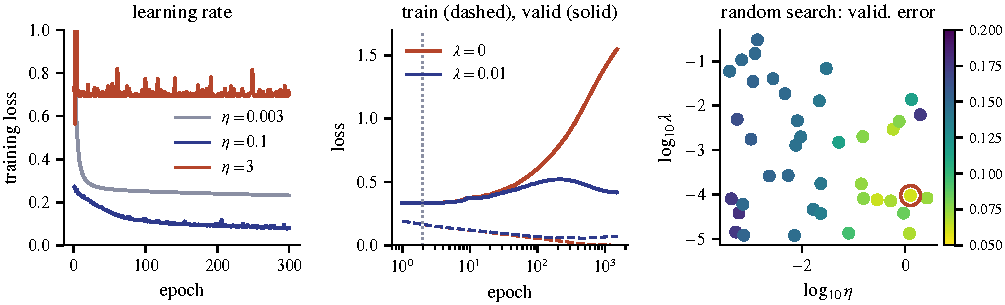
\includegraphics[width=\linewidth]{figures/n12_training.pdf}
\caption{Training ReLU networks on the two-moons data with Algorithm~\ref{alg:train} without early stopping (fixed
numbers of epochs; He initialisation, batches of 20 or 10). Left: training loss of a 2--64--64--1 network on 200 points for three learning rates; $\eta = 0.003$ is slow
($0.232$ after 300 epochs), $\eta = 0.1$ reaches $0.080$, and $\eta = 3$ jumps to a loss of $10.1$ in the third epoch
and then stays near $0.70$: every unit of the second hidden layer is dead, and the network outputs the same
probability, $0.40$, for every input (training error $47.5\%$). Centre: a 2--128--128--1 network on only 40 points
($\eta = 0.05$, log scale in epochs). Without weight decay the training loss falls to $0.001$ and the validation loss
rises to $1.55$ (validation error $16.8\%$); with $\lambda = 0.01$ it ends at $0.42$ (error $13.6\%$). The validation
loss is lowest, $0.33$, already at epoch~2 (dotted line), while the validation error of the $\lambda = 0$ run keeps
falling to its minimum, $14.9\%$, at epoch~202. Right: 40 trials of random search over
$\log_{10}\eta$ and $\log_{10}\lambda$ (60 epochs each, 2000 validation points); colour is validation error, the best
trial (circled, $6.05\%$) has $\eta \approx 1.3$, $\lambda \approx 10^{-4}$.}
\label{fig:training}
\end{figure}

\subsection{Weight decay}\label{sec:wd}

The $L_2$ penalty $\Omega(\theta) = \frac12\sum_k\norm{W^{(k)}}_F^2 = \frac12\sum_k\sum_{i,j}\big(W^{(k)}_{ij}\big)^2$
(the factor $\frac12$ only simplifies the gradient; Note~11, Section~7.1, omits it, so its $\lambda$ is half of
ours) adds
$\lambda W^{(k)}$ to each weight gradient, and a gradient step becomes
\begin{equation}\label{eq:wd}
  W^{(k)} \gets W^{(k)} - \eta\big(\nabla_{W^{(k)}}\ell + \lambda W^{(k)}\big) = (1 - \eta\lambda)\,W^{(k)} - \eta\,\nabla_{W^{(k)}}\ell :
\end{equation}
before each step every weight is multiplied by $1 - \eta\lambda$, hence the name \emph{weight decay}. It is ridge
regression's penalty (Note~8, Section~4.3) applied to every layer, and the MAP estimate under a Gaussian prior on the
weights (Note~8, Section~6). Two network-specific points:
\begin{itemize}
\item \emph{Biases are not penalised.} A bias shifts a unit's threshold; it does not make the function steeper or more
  complex, and penalising it would pull outputs towards zero for no reason (for instance away from the mean of the
  targets). Normalisation layers' scale and shift parameters (Section~\ref{sec:norm}) are usually exempt for the same
  reason.
\item \emph{With adaptive optimisers the decay must be decoupled.} Inside Adam the term $\lambda W$ would be rescaled
  per parameter; AdamW applies \eqref{eq:wd}'s shrinkage directly (Note~7, Section~6.4)~\cite{loshchilov2019}.
\end{itemize}
In the centre panel of Figure~\ref{fig:training}, $\lambda = 0.01$ keeps the validation loss at $0.42$ instead of
$1.55$, and the final validation error at $13.6\%$ instead of $16.8\%$.

\subsection{The \texorpdfstring{$L_1$}{L1} penalty}\label{sec:l1}

$\Omega(\theta) = \sum_k\sum_{i,j}|W^{(k)}_{ij}|$ has the (sub)gradient $\operatorname{sign}(W^{(k)})$, so each step moves
every weight towards zero by the \emph{constant} amount $\eta\lambda$, however small the weight already is. Weights whose
data gradient is weak reach zero. With the soft-thresholding update of Note~8, Section~5.1 (subtract $\eta\lambda$ in
absolute value and clip at zero) they stay exactly at zero, as in the lasso; a plain subgradient step instead makes them
oscillate around zero. The corresponding prior is the Laplace distribution. $L_1$ penalties on weights are used for pruning and interpretability, more rarely for accuracy.

\begin{worked}{5. Shrinking versus clipping to zero}
Take one weight $w = 0.5$ whose data gradient is zero (it does not help the fit), $\eta = 0.1$ and $\lambda = 0.5$.
\emph{$L_2$}: each step multiplies $w$ by $1 - \eta\lambda = 0.95$; after ten steps $w = 0.5 \times 0.95^{10} = 0.299$, and
it never reaches zero. \emph{$L_1$} with soft thresholding: each step subtracts $\eta\lambda = 0.05$; after ten steps
$w = 0$, and the clip keeps it there instead of letting an eleventh step overshoot to $-0.05$.
\end{worked}

\subsection{Dropout}\label{sec:dropout}

\emph{Dropout}~\cite{srivastava2014} regularises by injecting noise. During training, each hidden unit's output is set
to zero with probability $p_{\mathrm{d}}$, independently for each unit, each example and each step, and the surviving
units are scaled by $1/(1 - p_{\mathrm{d}})$ (``inverted'' dropout). With the mask $m_j \sim \text{Bernoulli}(1 -
p_{\mathrm{d}})$,
\[
  \tilde{h}_j = \frac{m_j\,h_j}{1 - p_{\mathrm{d}}}, \qquad \E[\tilde{h}_j] = \frac{(1 - p_{\mathrm{d}})\,h_j}{1 - p_{\mathrm{d}}} = h_j ,
\]
so the expected input of the next layer is unchanged, and at test time the network is used as it is, without masks or
rescaling. A unit can no longer rely on the presence of particular partners, which discourages fragile
co-adaptations; one can also view training as fitting an exponentially large family of thinned networks that share
weights, and the test-time network as an approximation to their average. Backpropagation through dropout multiplies the
upstream gradient by the same mask (Algorithm~\ref{alg:dropout}): a dropped unit passes no gradient.

\begin{algorithm}[H]
\caption{Inverted dropout on a layer's activations}\label{alg:dropout}
\begin{algorithmic}[1]
\Require activations $H \in \R^{n' \times H_k}$; drop probability $p_{\mathrm{d}} \in [0, 1)$; flag \emph{training}
\Function{DropoutForward}{$H$}
  \If{not \emph{training}} \Return $H$ \EndIf \Comment{inference: identity}
  \State $M_{ij} \gets \ind{u_{ij} > p_{\mathrm{d}}}/(1 - p_{\mathrm{d}})$ with $u_{ij} \sim \mathcal{U}(0, 1)$ \Comment{store $M$}
  \State \Return $M \odot H$
\EndFunction
\Function{DropoutBackward}{$\bar{H}_{\mathrm{out}}$} \Comment{adjoint of the output}
  \State \Return $M \odot \bar{H}_{\mathrm{out}}$
\EndFunction
\end{algorithmic}
\end{algorithm}

\begin{runtime}{dropout}
$O(n'H_k)$ random numbers and multiplications per layer and step, negligible next to the $O(n'H_kH_{k-1})$ matrix product;
memory $O(n'H_k)$ for the mask (often regenerated from the random seed instead of being stored). Zero cost at prediction.
Training usually needs more epochs, because the gradients are noisier.
\end{runtime}

\begin{worked}{6. A dropout sample}
Let $\hv = (2, 0, 1, 3)$ and $p_{\mathrm{d}} = 0.5$. The mask $(1, 0, 0, 1)$ gives $\tilde{\hv} = (4, 0, 0, 6)$. For a next-layer
unit with weights $(1, -1, 2, 1)$ the pre-activation is $4 + 0 + 0 + 6 = 10$ for this sample, while its expectation is
the undropped value $2 - 0 + 2 + 3 = 7$. Each $m_j/(1 - p_{\mathrm{d}})$ takes the values $0$ and $2$ with equal probability,
mean $1$ and variance $1$, so the dropout noise has variance $\sum_j w_j^2h_j^2 = 4 + 0 + 4 + 9 = 17$ (standard deviation
$4.1$). The network must learn to classify correctly despite this noise.
\end{worked}

\subsection{Early stopping and the bias--variance view}\label{sec:early}

All these penalties trade a little bias for a lower variance in the sense of Note~4, Section~6. The number of training
epochs is a capacity control of its own (Note~11, Section~7.2), and early stopping with patience (Note~7, Section~7.1)
is already part of Algorithm~\ref{alg:train}: it returns the parameters $\theta_{\text{best}}$ of the epoch with the
lowest validation loss, not the last ones. What is monitored matters. In the centre panel of
Figure~\ref{fig:training} the validation loss is lowest at epoch~2, because the cross-entropy punishes the network's
growing confidence on the points it gets wrong, while the validation error improves until about epoch~200; monitoring
the error, or using a patience of many epochs, avoids stopping too early. In practice one combines weight decay with
early stopping, and adds dropout when the network is large relative to the data. Data augmentation, the most effective
regulariser for images, is treated in Note~13, Section~6.

\section{Initialisation}\label{sec:init}

\paragraph{Biases} Biases are initialised to zero (or a small positive constant for ReLU units, so that they start
active). The interesting question is the weights.

\paragraph{Derivation: zero weights never move} Suppose all weights are zero in a network with tanh hidden
units and zero biases. Then every $\av^{(k)} = \vect{0}$, every hidden activation $\tanh 0 = 0$, and the output does not
depend on the input. In the backward pass, \eqref{eq:paramgrad} gives $\nabla_{W^{(k)}}\ell = \dv^{(k)}\hv^{(k-1)\mathsf{T}} =
0$ for every $k \ge 2$, because $\hv^{(k-1)} = \vect{0}$; and \eqref{eq:recursion} gives $\dv^{(k-1)} = g'(\vect{0}) \odot
(W^{(k)\mathsf{T}}\dv^{(k)}) = \vect{0}$, because $W^{(k)} = 0$, so $\nabla_{W^{(1)}}\ell = 0$ too. Only the output bias
gets a gradient. Gradient descent therefore never leaves the set where all weights and hidden biases are zero: only the
output bias moves, to the constant that best fits the targets, and the point it reaches is a stationary point (a saddle)
of $J$. With sigmoid hidden units $h = \sigma(0) = \frac12 \neq 0$, so the top-layer weights do receive gradients; but
all units of a layer stay identical, which is the symmetry problem treated next.

\paragraph{Derivation: equal weights stay equal} Suppose instead that two hidden units $i$ and $i'$ of layer $k$ start
with identical incoming weights and biases and identical outgoing weights. Then $a^{(k)}_i = a^{(k)}_{i'}$ for every
input, hence $h^{(k)}_i = h^{(k)}_{i'}$; in the backward pass $\delta^{(k)}_i = g'(a^{(k)}_i)\sum_r W^{(k+1)}_{ri}
\delta^{(k+1)}_r = \delta^{(k)}_{i'}$, so by \eqref{eq:paramgrad} their incoming weights receive identical gradients,
and so do their outgoing weights ($\delta^{(k+1)}_rh^{(k)}_i = \delta^{(k+1)}_rh^{(k)}_{i'}$). After the update they are
still identical, and by induction forever: the two units compute the same feature, and the layer has effectively
fewer units. Random initialisation \emph{breaks the symmetry}.

\paragraph{Derivation: the scale of the random weights} How large should the random weights be? Draw the $W_{ij}$ of
one layer independently with mean $0$ and variance $\sigma_w^2$, independent of the incoming activations, which we
take to have mean square $\E[h_j^2] = q$. Then, for a unit with $H_{k-1}$ inputs (its \emph{fan-in}) and zero bias,
\[
  \Var\big(a_i\big) = \sum_{j=1}^{H_{k-1}} \Var(W_{ij}h_j) = \sum_j \E[W_{ij}^2]\,\E[h_j^2] = H_{k-1}\,\sigma_w^2\,q ,
\]
since the products are uncorrelated with mean zero. The scale is preserved from layer to layer only if
$H_{k-1}\sigma_w^2 \approx 1$ (for activations that behave like the identity near zero, such as tanh) --- otherwise it
is multiplied by $H_{k-1}\sigma_w^2$ in every layer and grows or decays geometrically with depth. The same argument for
the backward pass \eqref{eq:recursion}, where $W\T$ sums over the $H_k$ units of the layer above (its \emph{fan-out}),
asks for $H_k\sigma_w^2 \approx 1$.
\begin{itemize}
\item \emph{Glorot (Xavier) initialisation}~\cite{glorot2010} compromises between the two conditions with
  $\sigma_w^2 = 2/(H_{k-1} + H_k)$; drawn uniformly from $[-b, b]$, whose variance is $b^2/3$, this gives
  $b = \sqrt{6/(H_{k-1} + H_k)}$.
\item \emph{He initialisation}~\cite{he2015} accounts for ReLU, which zeroes half of a symmetric input: if $a$ is
  symmetric about zero, $\E[\max(0, a)^2] = \frac12\Var(a)$, so $q$ is only half the previous layer's variance and the
  condition becomes $H_{k-1}\sigma_w^2 = 2$, i.e.\ $\sigma_w = \sqrt{2/H_{k-1}}$.
\end{itemize}

\begin{algorithm}[H]
\caption{Random initialisation of a fully connected network}\label{alg:init}
\begin{algorithmic}[1]
\Require layer widths $H_0, \dots, H_L$; scheme (Glorot for tanh/sigmoid, He for ReLU-type activations)
\Function{Initialise}{$H_0, \dots, H_L$}
  \For{$k = 1, \dots, L$}
    \If{Glorot} \ draw $W^{(k)}_{ij} \sim \mathcal{U}\big[-b, b\big]$, $b = \sqrt{6/(H_{k-1} + H_k)}$
    \Else \ draw $W^{(k)}_{ij} \sim \Normal\big(0, 2/H_{k-1}\big)$ \Comment{He}
    \EndIf
    \State $\bv^{(k)} \gets \vect{0}$
  \EndFor
  \State \Return $\theta$
\EndFunction
\end{algorithmic}
\end{algorithm}

\begin{runtime}{initialisation}
One random number per parameter: $O(p)$ time and the $O(p)$ memory of the parameters themselves. Negligible, but it
decides whether the first thousand steps make progress.
\end{runtime}

\begin{worked}{7. Numbers for a first layer}
A layer from $H_0 = 784$ inputs (a $28 \times 28$ image, standardised pixels) to $H_1 = 256$ units. \emph{Naive}:
$\sigma_w = 1$ gives $\Var(a) = 784$, a standard deviation of $28$; nearly every tanh unit is saturated, with
$g'(a) \approx 0$, and learns nothing. \emph{Glorot}: $b = \sqrt{6/1040} = 0.0760$, variance $2/1040 = 0.00192$, so
$\Var(a) = 784 \times 0.00192 = 1.51$. \emph{He}: $\sigma_w = \sqrt{2/784} = 0.0505$, so $\Var(a) = 2$ and, after the
ReLU, $\E[h^2] = 1$, the same mean square as the input.
\end{worked}

Figure~\ref{fig:init} follows the scale through 30 layers of width 256. For tanh, weights of standard deviation $1$
keep the pre-activations at a root mean square of about $16$ (85\% of units saturated, $|a| > 3$), while $0.01$
makes the signal vanish by a factor $0.16$ per layer; Glorot keeps it of order one, decaying slowly (from $1.0$ to
$0.12$ over 30 layers). For ReLU, Glorot's variance is half of what is needed and the mean square halves every layer, while
He initialisation keeps it roughly constant (from $1.41$ at layer~1 to $0.70$ at layer~30; the residual drift comes
from the finite width).

\begin{figure}[htbp]
\centering
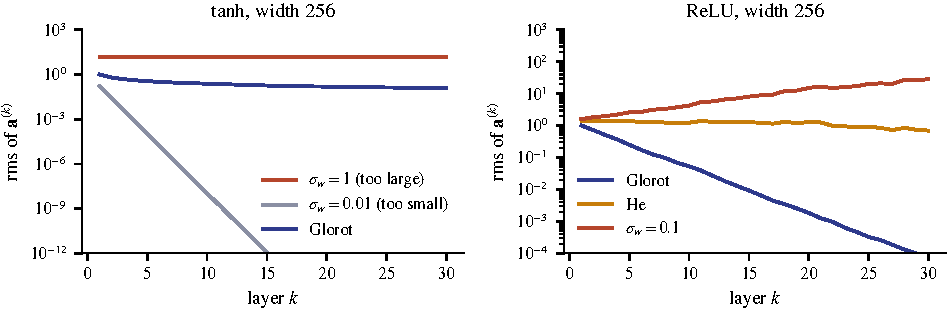
\includegraphics[width=\linewidth]{figures/n12_init.pdf}
\caption{Root mean square of the pre-activations $\av^{(k)}$ through a 30-layer fully connected network of width 256 at
initialisation (500 standard-normal inputs, zero biases, log scale). Left: tanh with weights of standard deviation 1,
0.01 and Glorot uniform. Right: ReLU with Glorot uniform, He, and a fixed standard deviation 0.1, slightly above He's
$\sqrt{2/256} = 0.088$, which multiplies the expected mean square by $256 \times 0.01/2 = 1.28$ per layer.}
\label{fig:init}
\end{figure}

\begin{physics}{signal propagation and the edge of chaos}
The variance recursion above is a mean-field theory: for a wide network, the pre-activations of a layer are
approximately Gaussian, and their variance $q_k$ obeys a deterministic map $q_k = \sigma_w^2\,\E[g(\sqrt{q_{k-1}}\,z)^2]
+ \sigma_b^2$ with $z \sim \Normal(0, 1)$, when the weights have variance $\sigma_w^2/H_{k-1}$ and the biases variance
$\sigma_b^2$. Poole \emph{et al.}~\cite{poole2016} and Schoenholz
\emph{et al.}~\cite{schoenholz2017} studied in the same way how the \emph{correlation} between the signals of two
different inputs evolves with depth. They found two phases, as in a magnet: an ordered phase, in which all inputs are
mapped to nearly the same representation and gradients vanish, and a chaotic phase, in which nearby inputs are driven
apart and gradients explode. Between them lies a critical line --- the ``edge of chaos'' --- where the depth scale over
which information survives diverges, like a correlation length at a critical point. Good initialisations place the
network at, or close to, criticality.
\end{physics}

\section{Choosing hyperparameters}\label{sec:hyper}

A network comes with many hyperparameters: the width and depth (Note~11, Section~7.2), the activation, the learning rate and its
schedule, the batch size, momentum or Adam's $\beta$'s, the weight decay $\lambda$, the dropout rate, the number of
epochs. They are chosen exactly as in Note~4, Section~7: train on $\Dtrain$, compare on $\Dvalid$, and report the final
error once on $\Dtest$. Two remarks:
\begin{itemize}
\item \emph{Search as in Note~4, Section~7.2}: log-uniform random draws of $\eta$ and $\lambda$ (they act
  multiplicatively), many short runs over wide ranges first, then longer runs in the good region, stopping clearly bad
  runs early. With five or more hyperparameters a grid is hopeless~\cite{bergstra2012}.
\item \emph{The learning rate usually matters most.} In the random search of Figure~\ref{fig:training} (right), the 20
  trials with $\eta < 0.01$ all end between $14.3\%$ and $17.85\%$ validation error after 60 epochs, while the 13 trials with
  $\eta \ge 0.1$ have a median of $7.45\%$; the weight decay matters much less over the range searched. Hyperparameters
  interact: the best learning rate depends on the batch size, the optimiser, the initialisation and the activation.
\end{itemize}

\section{Why training is hard}\label{sec:hard}

\subsection{Non-convexity and symmetries}\label{sec:nonconvex}

Note~11, Section~7.3, showed that the objective is not convex: permuting the hidden units of a layer (and, for tanh
units, negating a unit's incoming weights, bias and outgoing weights) leaves the function unchanged, so every minimiser
has $H!\,2^H$ equivalent copies, $3.7 \times 10^9$ for one tanh layer of 10 units. These copies are harmless --- all are
equally good --- and only show that ``the'' minimum does not exist.

What does hurt are regions where the gradient is small but the loss is not: \emph{plateaus}, where the loss barely
changes over long stretches (for example while many units are saturated), and \emph{saddle points}, which in high
dimension are far more common than poor local minima~\cite{dauphin2014} (Note~7, Section~4). On them, plain gradient
descent crawls; momentum, adaptive step sizes and mini-batch noise help to move on. Empirically, for large networks
the minima reached from different random initialisations are typically very similar in training loss, and usually in
test loss, although they are different points in parameter space~\cite[Section~8.2]{goodfellow2016}.

\subsection{Vanishing and exploding gradients}\label{sec:vanishing}

Unroll the recursion \eqref{eq:recursion} from the top to layer $1$. Each step multiplies by $W^{(k)\mathsf{T}}$ and by
$D^{(k-1)} = \diag\big(g'(\av^{(k-1)})\big)$:
\begin{equation}\label{eq:product}
  \dv^{(1)} = D^{(1)}W^{(2)\mathsf{T}}D^{(2)}W^{(3)\mathsf{T}}\cdots D^{(L-1)}W^{(L)\mathsf{T}}\,\dv^{(L)} ,
  \qquad
  \norm{\dv^{(1)}} \le \prod_{k=2}^{L}\Big(\norm{W^{(k)}}\,\max_j\big|g'(a^{(k-1)}_j)\big|\Big)\,\norm{\dv^{(L)}} ,
\end{equation}
with $\norm{W}$ the largest singular value. The gradient reaching the first layer is a product of $L - 1$ factors, and a
product of many factors is typically exponentially small or exponentially large: \emph{vanishing} or \emph{exploding
gradients}~\cite{bengio1994}. Sigmoid units are the worst case: $g' \le \frac14$, so unless the weights are large every
layer divides the signal by at least four. For a chain of ten sigmoid units with weights $1$, the factor is at most
$(1/4)^{10} = 9.5 \times 10^{-7}$: the first layers receive essentially no gradient and do not learn. Exploding
gradients appear when the factors exceed one, most dramatically in recurrent networks, where the same matrix is
multiplied in at every time step; gradient clipping (Note~7, Section~7) limits the damage.

Figure~\ref{fig:gradflow} measures the effect at initialisation in 30-layer networks of width 128. With sigmoid
units and Glorot weights the gradient at layer~1 is $5.5 \times 10^{-19}$ times that at layer~30; tanh with Glorot loses a
factor of five; ReLU with He initialisation keeps it of order one ($1.7$ times the top value), since $g' = 1$ on the
active units, and the residual network too ($2.0$ times).
The remedies are therefore: activations whose derivative is $1$ over a large range (ReLU and its smooth relatives GELU
and SiLU), initialisation at the right scale (Section~\ref{sec:init}), and the two architectural changes of
Sections~\ref{sec:norm} and~\ref{sec:residual}.

\begin{figure}[htbp]
\centering
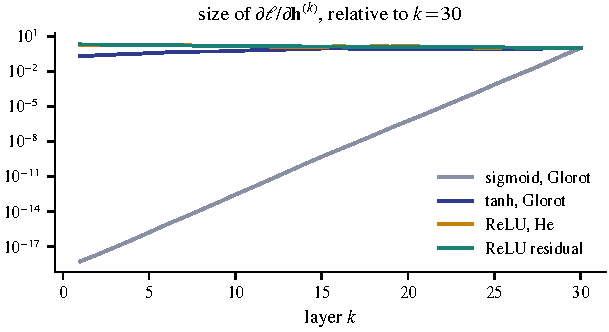
\includegraphics[width=0.64\linewidth]{figures/n12_gradflow.pdf}
\caption{Root mean square of $\partial\ell/\partial\hv^{(k)}$ in 30-layer networks of width 128 at initialisation (256 random inputs,
a random linear loss on the last layer), divided by its value at layer~30. The residual network adds each layer's output to
its input, $\hv^{(k)} = \hv^{(k-1)} + \mathrm{ReLU}(W^{(k)}\hv^{(k-1)})$, with He weights divided by $\sqrt{30}$.}
\label{fig:gradflow}
\end{figure}

\needspace{6\baselineskip}
\section{Practical tricks and the modern toolkit}\label{sec:practice}

\subsection{Inputs, optimiser and learning rate}\label{sec:tricks}

\paragraph{Standardise the inputs} Subtract the training mean of each input feature and divide by its standard
deviation, with training statistics only (Note~1, Section~5.1, on leakage). Features of very different scales make the
first-layer Hessian ill-conditioned, which slows gradient descent (Note~7, Section~3.2), and they break the
assumptions of the initialisation formulas~\cite{lecun1998}. Regression targets are standardised for the same reason.

\paragraph{Optimiser} Mini-batches of $32$ to a few thousand examples exploit vectorised hardware (Note~7, Section~5).
SGD with momentum (Note~7, Section~6.1) remains strong for convolutional networks; Adam and AdamW (Note~7, Section~6.4)
are the default elsewhere and are less sensitive to the learning rate. Newton's method (Note~7, Section~6.2) is out of
reach: the Hessian of a network with $p = 10^7$ parameters would have $10^{14}$ entries, and it is not positive definite away
from a minimum.

\paragraph{Learning-rate schedule} The learning rate is decreased during training with one of the schedules of
Note~7, Section~3.3; the Robbins--Monro conditions of Note~7, Section~5.3, say why a decay is needed for convergence
with noisy gradients. For example $\eta_t = \eta_0/t^{\delta}$ satisfies both conditions exactly when
$\frac12 < \delta \le 1$: the sum of $t^{-\delta}$ diverges for $\delta \le 1$, and the sum of $t^{-2\delta}$ converges
for $\delta > \frac12$. Warm-up matters most for deep networks with adaptive optimisers, because Adam's second-moment
estimate rests on very few gradients in the first steps. A rate that is too large can do more than oscillate: in the
left panel of Figure~\ref{fig:training}, one huge step with $\eta = 3$ kills every ReLU unit of the second hidden
layer, and the network is left predicting a constant (loss $\approx 0.70$; compare Question~A5).

\subsection{Normalisation layers}\label{sec:norm}

Initialisation fixes the scale of the signals at the start; normalisation layers keep it fixed throughout training.
\emph{Batch normalisation}~\cite{ioffe2015} standardises each unit's pre-activation over the mini-batch and then
restores a learned scale and shift:
\begin{equation}\label{eq:bn}
  \hat{a}_{ij} = \frac{a_{ij} - \mu_j}{\sqrt{s_j^2 + \epsilon}}, \qquad
  \mu_j = \frac1{n'}\sum_{i \in B}a_{ij}, \quad s_j^2 = \frac1{n'}\sum_{i \in B}(a_{ij} - \mu_j)^2, \qquad
  \tilde{a}_{ij} = \gamma_j\,\hat{a}_{ij} + \beta_j ,
\end{equation}
for example $i$ and unit $j$, with a small $\epsilon$ (e.g.\ $10^{-5}$) against division by zero. The parameters
$\gamma_j, \beta_j$ are trained with the rest, so the layer can represent any scale, including the identity; the bias of
the preceding affine layer becomes redundant (the mean is subtracted) and is dropped. At test time a prediction must not
depend on the other examples in the batch, so $\mu_j$ and $s_j^2$ are replaced by running averages accumulated during
training. Batch normalisation allows much larger learning rates; it was introduced to reduce shifts of the input
distribution of each layer during training, and later work argues that its main benefit is a smoother loss
landscape~\cite{santurkar2018}. Its dependence on the batch is also its weakness: small batches give noisy statistics,
and training and test behaviour differ.

\emph{Layer normalisation}~\cite{ba2016} applies the same standardisation to the $H$ units of \emph{one} example, with
$\mu_i$ and $s_i^2$ computed over $j$; it behaves identically for any batch size, at training and test time, and is the
normalisation of transformers. RMSNorm divides by the root mean square without subtracting the mean, a cheaper
variant~\cite{zhang2019} used in several recent language models~\cite{touvron2023}.

\begin{algorithm}[H]
\caption{Batch normalisation and layer normalisation (forward pass)}\label{alg:norm}
\begin{algorithmic}[1]
\Require pre-activations $A \in \R^{n' \times H}$; scale and shift $\vect{\gamma}, \vect{\beta} \in \R^H$; $\epsilon > 0$;
  running averages $\bar{\mu}, \bar{s}^2$ and their decay $\rho$ (batch norm only)
\Function{BatchNorm}{$A$, \emph{training}}
  \If{\emph{training}}
    \State $\mu_j \gets$ mean of column $j$, \ $s_j^2 \gets$ variance of column $j$ \Comment{over the $n'$ examples}
    \State $\bar{\mu} \gets \rho\bar{\mu} + (1 - \rho)\mu$, \ $\bar{s}^2 \gets \rho\bar{s}^2 + (1 - \rho)s^2$ \Comment{for inference}
  \Else \ $\mu \gets \bar{\mu}$, \ $s^2 \gets \bar{s}^2$
  \EndIf
  \State \Return $\tilde{A}_{ij} = \gamma_j(A_{ij} - \mu_j)/\sqrt{s_j^2 + \epsilon} + \beta_j$
\EndFunction
\Function{LayerNorm}{$A$} \Comment{same at training and test time}
  \State $\mu_i \gets$ mean of row $i$, \ $s_i^2 \gets$ variance of row $i$ \Comment{over the $H$ units}
  \State \Return $\tilde{A}_{ij} = \gamma_j(A_{ij} - \mu_i)/\sqrt{s_i^2 + \epsilon} + \beta_j$
\EndFunction
\end{algorithmic}
\end{algorithm}

\begin{runtime}{normalisation layers}
Forward: $O(n'H)$ per layer (two passes for mean and variance, one to normalise); backward, obtained by automatic
differentiation, also $O(n'H)$. Both are small next to the $O(n'HH')$ matrix product of the layer. Memory: the normalised
values and the $n'$ or $H$ statistics for the backward pass, $2H$ parameters, and for batch norm $2H$ running averages.
Prediction: $O(H)$ per example (batch norm at inference is an affine map and can be folded into the preceding weights).
\end{runtime}

\begin{worked}{8. Normalising four numbers}
One unit has the pre-activations $(1, 2, 3, 6)$ on a mini-batch of four examples. Mean $\mu = 3$, variance
$s^2 = \frac14(4 + 1 + 0 + 9) = 3.5$, standard deviation $1.871$ (take $\epsilon \approx 0$). The normalised values are
$(-1.069, -0.535, 0, 1.604)$: mean $0$, variance $1$. With $\gamma = 2$ and $\beta = 1$ the layer outputs
$(-1.138, -0.069, 1, 4.207)$. Layer normalisation does the same arithmetic on the four units of \emph{one} example: if
an example's pre-activations were $(1, 2, 3, 6)$, it would produce the same numbers if every unit had $\gamma_j = 2$
and $\beta_j = 1$, whatever the other examples in the batch.
\end{worked}

\subsection{Residual connections}\label{sec:residual}

A \emph{residual block}~\cite{he2016} adds its input to its output:
\begin{equation}\label{eq:residual}
  \hv^{(k)} = \hv^{(k-1)} + F_k\big(\hv^{(k-1)}\big) ,
\end{equation}
where $F_k$ is a small sub-network (for example normalisation, affine, activation, affine). The block learns the
\emph{change} $F_k$ to the representation rather than a whole new representation, and if $F_k = 0$ it is the identity,
so adding blocks can never make the best achievable fit worse.

\paragraph{Derivation: an identity path for the gradient} Differentiating \eqref{eq:residual},
$\partial\hv^{(k)}/\partial\hv^{(k-1)} = I + \partial F_k/\partial\hv^{(k-1)}$, so the backward recursion reads
\[
  \frac{\partial\ell}{\partial\hv^{(k-1)}} = \frac{\partial\ell}{\partial\hv^{(k)}} +
  \Big(\frac{\partial F_k}{\partial\hv^{(k-1)}}\Big)^{\!\mathsf{T}}\frac{\partial\ell}{\partial\hv^{(k)}} .
\]
The first term copies the gradient unchanged to the layer below. Unrolling over all blocks, the product of
Jacobians $\prod_k (I + J_k)$ expands into a sum of products of all subsets of the $J_k$, including the term $I$: the
gradient at the bottom contains $\partial\ell/\partial\hv^{(L)}$ itself, however deep the network. In one dimension with
twenty blocks, each of slope $J_k = 0.1$, a plain chain multiplies the gradient by $0.1^{20} = 10^{-20}$, the residual
chain by $1.1^{20} = 6.7$; with $J_k = -0.1$ the residual factor is $0.9^{20} = 0.12$ --- smaller, but not exponentially
small in the way the plain chain is. Residual connections made networks of a hundred layers and more
trainable~\cite{he2016}; Note~13, Section~7, shows them in convolutional networks.

\begin{algorithm}[H]
\caption{A pre-normalisation residual MLP block (forward and backward)}\label{alg:resblock}
\begin{algorithmic}[1]
\Require block input $X \in \R^{n' \times H}$; LayerNorm parameters; $W_1 \in \R^{H_{\mathrm{f}} \times H}$, $W_2 \in
  \R^{H \times H_{\mathrm{f}}}$ and biases; activation $g$ (e.g.\ GELU)
\Function{ResBlockForward}{$X$}
  \State $Z \gets \Call{LayerNorm}{X}$; \ $A \gets ZW_1\T + \onev\bv_1\T$; \ $U \gets g(A)$; \ $F \gets UW_2\T + \onev\bv_2\T$
  \State \Return $X + F$ \Comment{the skip connection}
\EndFunction
\Function{ResBlockBackward}{$\bar{Y}$} \Comment{$\bar{Y} = \partial\ell/\partial(\text{output})$}
  \State $\bar{F} \gets \bar{Y}$; \ gradients of $W_2, \bv_2$ from $\bar{F}$ and $U$ as in \eqref{eq:matrix}; \ $\bar{A} \gets (\bar{F} W_2) \odot g'(A)$
  \State gradients of $W_1, \bv_1$ from $\bar{A}$ and $Z$; \ $\bar{Z} \gets \bar{A} W_1$; \ $\bar{X}_F \gets$ LayerNorm backward of $\bar{Z}$
  \State \Return $\bar{X} = \bar{Y} + \bar{X}_F$ \Comment{identity path plus branch}
\EndFunction
\end{algorithmic}
\end{algorithm}

\begin{runtime}{residual MLP block}
Forward: two matrix products, $O(n'HH_{\mathrm{f}})$ each, plus $O(n'(H + H_{\mathrm{f}}))$ for the normalisation, activation
and addition; backward about twice the forward. Parameters: $2HH_{\mathrm{f}} + H_{\mathrm{f}} + 3H$. The skip connection
itself costs $O(n'H)$ and no parameters. In transformers $H_{\mathrm{f}} = 4H$ is the usual choice.
\end{runtime}

\begin{modern}{the training recipe of a transformer}
A transformer layer consists of two residual blocks, $\x \gets \x + \mathrm{Attention}(\mathrm{LN}(\x))$ and
$\x \gets \x + \mathrm{MLP}(\mathrm{LN}(\x))$, where the MLP is the GELU block of Algorithm~\ref{alg:resblock}. Putting the
normalisation inside the branch (``pre-LN''), so that the skip path is a pure identity, trains more stably than the
original arrangement with the normalisation after the addition and tolerates shorter warm-ups~\cite{xiong2020}. The
rest of the recipe --- AdamW, warm-up and cosine decay, gradient clipping --- is that of Note~7, Section~7; what this
note adds is the initialisation, the placement of the normalisation, mixed precision, and weight decay that skips biases
and normalisation parameters. Nothing in this pipeline is specific to language: the same recipe trains vision
transformers and the networks used for physics surrogates.
\end{modern}

\subsection{A debugging checklist}\label{sec:debug}

Networks fail silently. The following order of checks catches most problems before an expensive run.
\begin{enumerate}
\item \emph{Look at the data and the pipeline.} Plot inputs and labels after preprocessing; check shapes, units,
  standardisation with training statistics, and that labels are aligned with inputs.
\item \emph{Check the initial loss.} With small output weights an $m$-class softmax predicts nearly uniform
  probabilities, so the initial cross-entropy should be close to $\ln m$ ($2.303$ for ten classes). A much larger value
  means badly scaled outputs or a wrong loss.
\item \emph{Check the gradient} on a tiny network (Section~\ref{sec:gradcheck}) if any backward code was written by hand.
\item \emph{Overfit a tiny subset.} Train on 10 to 100 examples without regularisation. The training loss must go close
  to zero; if it does not, the model, the loss or the optimiser is broken, and no amount of data will fix it.
\item \emph{Find the learning rate.} Try a few values a factor of three to ten apart; take the largest that decreases the
  loss smoothly (Figure~\ref{fig:training}, left).
\item \emph{Watch the curves.} Plot training and validation loss per epoch (Figure~\ref{fig:training}, centre). Training loss
  high: underfitting --- bigger model, longer training, higher learning rate. Gap growing: overfitting --- more data or
  augmentation, weight decay, dropout, early stopping. Also monitor the gradient norm and the fraction of inactive ReLU
  units per layer.
\item \emph{Only then scale up}, and change one thing at a time.
\end{enumerate}

\begin{physics}{physics-informed training}
Automatic differentiation computes derivatives not only with respect to parameters but also with respect to
\emph{inputs}. Physics-informed neural networks~\cite{raissi2019} exploit this: a network $u_\theta(x, t)$ represents the
solution of a differential equation, say $\partial_t u = \nu\,\partial_x^2u$, and the training loss adds to the data misfit
the squared residual $\big(\partial_tu_\theta - \nu\,\partial_x^2u_\theta\big)^2$ at many collocation points, with the
derivatives obtained by differentiating the network through its graph. Training then uses exactly
Algorithm~\ref{alg:train}, and all the issues of this note reappear --- the residual and data terms have very different
scales and gradient magnitudes, and balancing them is one of the main practical difficulties of the method. Smooth
activations such as tanh or SiLU are used, because the second derivative of a ReLU network is zero almost everywhere.
\end{physics}

\begin{keyidea}[Summary]
Training a network is regularised empirical risk minimisation with mini-batch gradients. For matched output/loss pairs
the output error is $\yv - \tvec$. Backpropagation applies the chain rule in reverse order: the error of layer $k - 1$ is
$g'(\av^{(k-1)}) \odot W^{(k)\mathsf{T}}\dv^{(k)}$ and the weight gradient is the outer product $\dv^{(k)}\hv^{(k-1)\mathsf{T}}$; a
training step costs about three forward passes, and the price is the memory of the stored activations. Automatic
differentiation does the same for any graph of modules; central differences check it. Weight decay shrinks weights (not
biases) by $1 - \eta\lambda$ per step, $L_1$ drives some to zero, dropout injects scaled multiplicative noise, and early
stopping limits the number of steps. Weights must be random, to break symmetry, with variance about
$2/(\text{fan-in} + \text{fan-out})$ (Glorot) or $2/\text{fan-in}$ for ReLU (He). The loss is non-convex and full of symmetric copies, plateaus and saddles;
gradients vanish or explode as products of many Jacobians. ReLU-type activations, good initialisation, normalisation
layers and residual connections keep the gradients alive, and a disciplined checklist --- initial loss, tiny-subset
overfitting, learning-rate sweep, learning curves --- keeps the training honest.
\end{keyidea}

\begin{questions}
\begin{conceptual}
\item List the four ingredients that stochastic gradient descent needs before it can train a neural network, and say in
  one sentence why each is needed.
\item Every row of the softmax Jacobian sums to zero, and the components of $\yv - \tvec$ sum to zero. Explain why these
  are two statements of the same fact.
\item In Worked example~2 the input $x$ has two children. What would go wrong if the backward sweep overwrote $\bar{x}$
  instead of accumulating it, and why does the same accumulation make shared weights correct?
\item What must be stored during the forward pass so that the backward pass can run? How does this memory grow with the
  batch size and the depth, and what does activation checkpointing trade for it?
\item In Worked example~3 hidden unit~1 receives no gradient. Under which condition does this persist across all
  training examples, and can the unit then recover? How do He initialisation and a small positive bias change the odds,
  and how can a too-large learning rate cause the situation (Figure~\ref{fig:training}, left)?
\item In gradient checking, why are central differences preferred to forward differences, why is a relative error used,
  and why should dropout be switched off? Why may a correct implementation disagree on a few coordinates with ReLU units?
\item Why are biases usually excluded from weight decay? Why must weight decay be decoupled from the gradient when Adam is
  used?
\item Compare what the $L_2$ and $L_1$ penalties do to a weight whose data gradient is zero under repeated gradient
  steps. Why does the $L_1$ penalty need a clip-at-zero update to produce exact zeros?
\item In inverted dropout, why are the surviving activations divided by $1 - p_{\mathrm{d}}$? What would go wrong at test
  time if a network trained with dropout but without this rescaling were used without masks?
\item Explain why a tanh network cannot be trained from all-zero weights, and why initialising all weights to the same
  non-zero constant is not much better.
\item State the variance condition behind Glorot initialisation and explain where the extra factor $2$ in He
  initialisation comes from.
\item Why are plateaus and saddle points, rather than poor local minima, the main obstacle when training large networks,
  and which ingredients of stochastic gradient training help to leave them?
\item Using \eqref{eq:product}, explain why deep networks of sigmoid units suffer from vanishing gradients, and list three
  remedies discussed in this note.
\item How does batch normalisation behave differently at training and at test time, and why? Give two reasons why layer
  normalisation is preferred in transformers.
\item Explain, using the Jacobian of a residual block, why gradients reach the first layers of a very deep residual network.
\item A ten-class classifier starts training with a cross-entropy of $23$ instead of about $2.3$. What does this suggest?
  In what order would you then carry out the checks of Section~\ref{sec:debug}, and why is overfitting a tiny subset a
  useful test?
\item In the random search of Figure~\ref{fig:training} (right), which hyperparameter mattered most? Why do interactions
  between hyperparameters (for example the learning rate and the batch size) argue against tuning them one at a time?
\item Explain why the number of training epochs acts as a capacity control. In Algorithm~\ref{alg:train}, what does the
  patience $P$ control, and why is $\theta_{\text{best}}$ returned rather than the final $\theta$? In the centre panel of
  Figure~\ref{fig:training}, why would monitoring the validation loss with a small patience stop too early?
\item Why does mixed-precision training keep a 32-bit copy of the weights, and why does multiplying the loss by a constant
  before the backward pass not change the direction of the gradient?
\end{conceptual}

\begin{calculations}
\item A softmax output is $\yv = (0.1, 0.2, 0.7)$. Write the $3 \times 3$ Jacobian $\partial\yv/\partial\av$ and verify
  that its rows sum to zero. For the true class $3$, compute $\partial\ell/\partial\yv$ for the cross-entropy, multiply
  it by the Jacobian to obtain $\dv = \partial\ell/\partial\av$, and check the result against $\yv - \tvec$.
\item A 2--2--1 network has ReLU hidden units with $W^{(1)} = \begin{pmatrix} 1 & -1 \\ -1 & 1\end{pmatrix}$, $\bv^{(1)} = \vect{0}$,
  and a sigmoid output with $W^{(2)} = (2, 1)$, $b^{(2)} = -1$, trained with the binary cross-entropy. For $\x = (2, 1)$ and
  $t = 0$ carry out the forward pass (pre-activations, activations, output, loss) and the backward pass: $\delta^{(2)}$,
  $\dv^{(1)}$, and the gradients of all weights and biases. Which parameters receive a zero gradient, and why?
\item For $f(x, y, z) = (x + y)\,z + x^2$ draw the computational graph with intermediate nodes $u = x + y$, $v = uz$,
  $w = x^2$, $f = v + w$. At $(x, y, z) = (1, 2, -1)$ compute all values in a forward sweep and all adjoints in one backward
  sweep, and check them against the partial derivatives computed directly.
\item A backprop gradient $\gvec_{\mathrm{bp}} = (0.50, -1.20, 0.003)$ is compared with a finite-difference gradient
  $\gvec_{\mathrm{fd}} = (0.50, -1.19, 0.004)$. Compute $r$ of \eqref{eq:relerr} over the three coordinates, and the same
  ratio $|g_{\mathrm{bp}} - g_{\mathrm{fd}}|/(|g_{\mathrm{bp}}| + |g_{\mathrm{fd}}|)$ for each coordinate separately.
  Which coordinate is suspicious, and how could a ReLU kink explain a disagreement on one coordinate even when the code
  is correct?
\item Return to Worked example~3 and take a step with $\eta = 0.1$ instead of $0.05$. Compute the new parameters, the new
  forward pass and the new loss. What happened to hidden unit~2, and what gradient will its weights receive at the next
  step on this example?
\item A weight $w = 0.3$ has zero data gradient. With $\eta = 0.1$ and $\lambda = 1$, how many steps does it take for the
  $L_1$ penalty to set it to zero, and what is its value after the same number of steps with weight decay
  \eqref{eq:wd}?
\item A fully connected layer has $512$ inputs and $512$ outputs. Compute the Glorot bound $b$ and the He standard
  deviation. If instead the weights have standard deviation $0.1$ and the inputs have unit mean square, what is the
  standard deviation of a pre-activation? With this standard deviation, by what factor does the mean square $\E[h^2]$
  of the hidden activations grow per ReLU layer (use $\E[h^2] = \frac12\Var(a)$), and after how many layers has it grown
  by more than $10^3$?
\item One unit of a batch-normalisation layer receives the pre-activations $(2, 4, 4, 6)$ on a mini-batch, and has $\gamma
  = 3$, $\beta = -1$, $\epsilon \approx 0$. Compute the batch mean and variance, the normalised values and the outputs.
  At test time the running averages are $\bar{\mu} = 3.8$ and $\bar{s}^2 = 2.25$; what is the output for a pre-activation of $5$?
\end{calculations}

\begin{derivations}
\item Derive the Jacobian $\partial\yv/\partial\av = \diag(\yv) - \yv\yv\T$ of the softmax and use it to show
  $\partial\ell/\partial\av = \yv - \tvec$ for the cross-entropy. Show that for $m = 2$ the result reduces to the
  sigmoid case $y - t$ of Note~9.
\item Starting from the per-example recursion \eqref{eq:recursion}--\eqref{eq:paramgrad}, derive the mini-batch
  equations \eqref{eq:matrix} for the mean loss, and count the multiply-adds of the forward and backward passes to show
  that a training step costs about three forward passes.
\item Derive the variance recursion for the pre-activations of a network with independent zero-mean weights. Show that
  $\E[\max(0, a)^2] = \frac12\Var(a)$ when $a$ is symmetric about zero, and obtain the He condition. Repeat the argument
  for the backward pass to obtain the fan-out condition, and explain Glorot's compromise.
\item Prove that gradient descent started from all-zero weights and biases in a tanh network changes only the output
  bias, and that with a small enough learning rate it converges to a stationary point of the training objective. Then prove by induction that two hidden units with identical incoming and outgoing
  weights remain identical under gradient descent.
\item For a stack of $L$ residual blocks \eqref{eq:residual} with Jacobians $J_k = \partial F_k/\partial\hv^{(k-1)}$, write
  $\partial\ell/\partial\hv^{(0)}$ as a product and expand it as a sum over subsets of blocks. Compare with a plain stack,
  and discuss what happens when all $J_k$ are small.
\end{derivations}

\begin{programming}
\item Implement Algorithm~\ref{alg:backprop} in numpy for an MLP with ReLU hidden layers and a softmax output, and verify it
  with Algorithm~\ref{alg:gradcheck}. Then introduce three deliberate bugs (a missing $g'$, a missing transpose that happens
  to have the right shape for square layers, a batch mean replaced by a sum) and report the relative error each produces.
\item Reproduce Figures~\ref{fig:init} and~\ref{fig:gradflow} in numpy. Add batch normalisation (Algorithm~\ref{alg:norm})
  before each activation of the sigmoid network and measure again how the gradient changes with depth.
\item In PyTorch, train an MLP on the two-moons data (or MNIST) with AdamW, linear warm-up and cosine decay. (a)~First
  check the initial loss and overfit 50 examples. (b)~Run a random search of 30 trials over $\log_{10}\eta$, $\log_{10}\lambda$
  and the dropout rate, and plot the validation error against each hyperparameter. Which matters most? (c)~Compare the
  validation curves of the best setting with and without weight decay and dropout.
\end{programming}
\end{questions}

\paragraph{Further reading} Goodfellow, Bengio and Courville~\cite{goodfellow2016}, chapters~6--8; Prince~\cite{prince2023},
chapters~7--9 and~11; Bishop~\cite{bishop2006}, chapter~5; Murphy~\cite{murphy2022}, chapter~13; Baydin
\emph{et al.}~\cite{baydin2018} on automatic differentiation; LeCun \emph{et al.}~\cite{lecun1998} for practical advice
that is still valid.

\begin{thebibliography}{99}\small
\bibitem{ba2016} J.~L. Ba, J.~R. Kiros and G.~E. Hinton, Layer normalization, arXiv:1607.06450 (2016).
\bibitem{baydin2018} A.~G. Baydin, B.~A. Pearlmutter, A.~A. Radul and J.~M. Siskind, Automatic differentiation in machine learning: a survey, \emph{J.\ Mach.\ Learn.\ Res.}\ 18(153), 1--43 (2018).
\bibitem{bengio1994} Y.~Bengio, P.~Simard and P.~Frasconi, Learning long-term dependencies with gradient descent is difficult, \emph{IEEE Trans.\ Neural Netw.}\ 5(2), 157--166 (1994).
\bibitem{bergstra2012} J.~Bergstra and Y.~Bengio, Random search for hyper-parameter optimization, \emph{J.\ Mach.\ Learn.\ Res.}\ 13, 281--305 (2012).
\bibitem{bishop2006} C.~M. Bishop, \emph{Pattern Recognition and Machine Learning}, Springer (2006).
\bibitem{chen2016} T.~Chen, B.~Xu, C.~Zhang and C.~Guestrin, Training deep nets with sublinear memory cost, arXiv:1604.06174 (2016).
\bibitem{dauphin2014} Y.~N. Dauphin, R.~Pascanu, C.~Gulcehre, K.~Cho, S.~Ganguli and Y.~Bengio, Identifying and attacking the saddle point problem in high-dimensional non-convex optimization, \emph{NeurIPS} (2014).
\bibitem{glorot2010} X.~Glorot and Y.~Bengio, Understanding the difficulty of training deep feedforward neural networks, \emph{Proc.\ AISTATS}, 249--256 (2010).
\bibitem{goodfellow2016} I.~Goodfellow, Y.~Bengio and A.~Courville, \emph{Deep Learning}, MIT Press (2016).
\bibitem{he2015} K.~He, X.~Zhang, S.~Ren and J.~Sun, Delving deep into rectifiers: surpassing human-level performance on ImageNet classification, \emph{Proc.\ ICCV}, 1026--1034 (2015).
\bibitem{he2016} K.~He, X.~Zhang, S.~Ren and J.~Sun, Deep residual learning for image recognition, \emph{Proc.\ CVPR}, 770--778 (2016).
\bibitem{ioffe2015} S.~Ioffe and C.~Szegedy, Batch normalization: accelerating deep network training by reducing internal covariate shift, \emph{ICML} (2015).
\bibitem{lecun1998} Y.~LeCun, L.~Bottou, G.~B. Orr and K.-R. M\"uller, Efficient BackProp, in \emph{Neural Networks: Tricks of the Trade}, Lecture Notes in Computer Science 1524, Springer, 9--50 (1998).
\bibitem{loshchilov2019} I.~Loshchilov and F.~Hutter, Decoupled weight decay regularization, \emph{ICLR} (2019).
\bibitem{micikevicius2018} P.~Micikevicius \emph{et al.}, Mixed precision training, \emph{ICLR} (2018).
\bibitem{murphy2022} K.~P. Murphy, \emph{Probabilistic Machine Learning: An Introduction}, MIT Press (2022).
\bibitem{plessix2006} R.-E. Plessix, A review of the adjoint-state method for computing the gradient of a functional with geophysical applications, \emph{Geophys.\ J.\ Int.}\ 167, 495--503 (2006).
\bibitem{poole2016} B.~Poole, S.~Lahiri, M.~Raghu, J.~Sohl-Dickstein and S.~Ganguli, Exponential expressivity in deep neural networks through transient chaos, \emph{NeurIPS} (2016).
\bibitem{prince2023} S.~J.~D. Prince, \emph{Understanding Deep Learning}, MIT Press (2023).
\bibitem{raissi2019} M.~Raissi, P.~Perdikaris and G.~E. Karniadakis, Physics-informed neural networks: a deep learning framework for solving forward and inverse problems involving nonlinear partial differential equations, \emph{J.\ Comput.\ Phys.}\ 378, 686--707 (2019).
\bibitem{rumelhart1986} D.~E. Rumelhart, G.~E. Hinton and R.~J. Williams, Learning representations by back-propagating errors, \emph{Nature} 323, 533--536 (1986).
\bibitem{santurkar2018} S.~Santurkar, D.~Tsipras, A.~Ilyas and A.~M\k{a}dry, How does batch normalization help optimization?, \emph{NeurIPS} (2018).
\bibitem{schoenholz2017} S.~S. Schoenholz, J.~Gilmer, S.~Ganguli and J.~Sohl-Dickstein, Deep information propagation, \emph{ICLR} (2017).
\bibitem{srivastava2014} N.~Srivastava, G.~Hinton, A.~Krizhevsky, I.~Sutskever and R.~Salakhutdinov, Dropout: a simple way to prevent neural networks from overfitting, \emph{J.\ Mach.\ Learn.\ Res.}\ 15, 1929--1958 (2014).
\bibitem{touvron2023} H.~Touvron \emph{et al.}, LLaMA: open and efficient foundation language models, arXiv:2302.13971 (2023).
\bibitem{xiong2020} R.~Xiong \emph{et al.}, On layer normalization in the transformer architecture, \emph{ICML} (2020).
\bibitem{zhang2019} B.~Zhang and R.~Sennrich, Root mean square layer normalization, \emph{NeurIPS} (2019).
\end{thebibliography}

\SourceNote
{\footnotesize\color{mute}The IFT~6390 slides on training neural networks are based on material by Hugo Larochelle.\par}
\end{document}
